\documentclass[tikz,border=10pt]{standalone}
\usepackage{amsmath}
\begin{document}
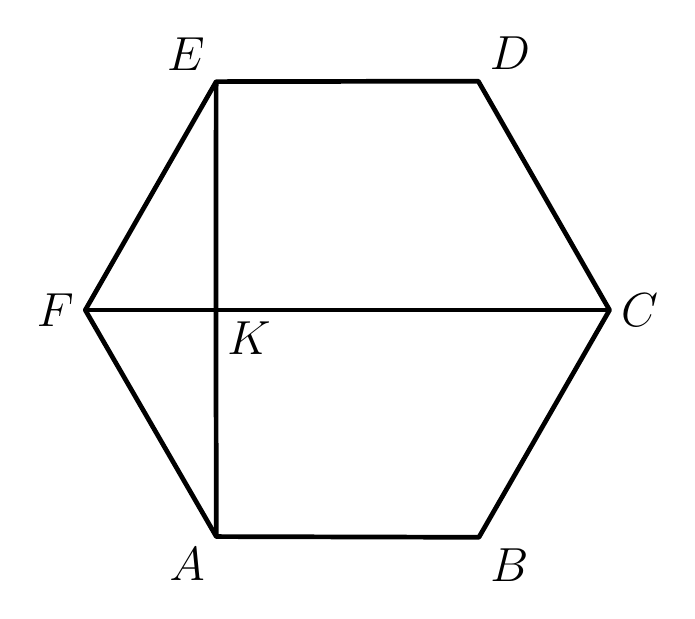
\begin{tikzpicture}[line width=1.7pt, line join=round]
\coordinate (A) at (-1.682,-2.866);
\coordinate (B) at (1.653,-2.875);
\coordinate (C) at (3.312,0.011);
\coordinate (D) at (1.645,2.918);
\coordinate (F) at (-3.346,0.011);
\coordinate (K) at (-1.687,0.011);



\coordinate (E) at (-1.684,2.912);


\draw (A) -- (B) -- (C) -- (D) -- (E) -- (F) -- cycle;


\draw (F) -- (K) -- (C);
\draw (E) -- (K) -- (A);


\node[above left] at (E) {\fontsize{17}{20.4}\selectfont $E$};
\node[above right] at (D) {\fontsize{17}{20.4}\selectfont $D$};
\node[below left] at (A) {\fontsize{17}{20.4}\selectfont $A$};
\node[below right] at (B) {\fontsize{17}{20.4}\selectfont $B$};
\node[left] at (F) {\fontsize{17}{20.4}\selectfont $F$};
\node[below right] at (K) {\fontsize{17}{20.4}\selectfont $K$};
\node[right] at (C) {\fontsize{17}{20.4}\selectfont $C$};
\end{tikzpicture}
\end{document}